\documentclass[1p]{elsarticle_modified}
%\bibliographystyle{elsarticle-num}

%\usepackage[colorlinks]{hyperref}
%\usepackage{abbrmath_seonhwa} %\Abb, \Ascr, \Acal ,\Abf, \Afrak
\usepackage{amsfonts}
\usepackage{amssymb}
\usepackage{amsmath}
\usepackage{amsthm}
\usepackage{scalefnt}
\usepackage{amsbsy}
\usepackage{kotex}
\usepackage{caption}
\usepackage{subfig}
\usepackage{color}
\usepackage{graphicx}
\usepackage{xcolor} %% white, black, red, green, blue, cyan, magenta, yellow
\usepackage{float}
\usepackage{setspace}
\usepackage{hyperref}

\usepackage{tikz}
\usetikzlibrary{arrows}

\usepackage{multirow}
\usepackage{array} % fixed length table
\usepackage{hhline}

%%%%%%%%%%%%%%%%%%%%%
\makeatletter
\renewcommand*\env@matrix[1][\arraystretch]{%
	\edef\arraystretch{#1}%
	\hskip -\arraycolsep
	\let\@ifnextchar\new@ifnextchar
	\array{*\c@MaxMatrixCols c}}
\makeatother %https://tex.stackexchange.com/questions/14071/how-can-i-increase-the-line-spacing-in-a-matrix
%%%%%%%%%%%%%%%

\usepackage[normalem]{ulem}

\newcommand{\msout}[1]{\ifmmode\text{\sout{\ensuremath{#1}}}\else\sout{#1}\fi}
%SOURCE: \msout is \stkout macro in https://tex.stackexchange.com/questions/20609/strikeout-in-math-mode

\newcommand{\cancel}[1]{
	\ifmmode
	{\color{red}\msout{#1}}
	\else
	{\color{red}\sout{#1}}
	\fi
}

\newcommand{\add}[1]{
	{\color{blue}\uwave{#1}}
}

\newcommand{\replace}[2]{
	\ifmmode
	{\color{red}\msout{#1}}{\color{blue}\uwave{#2}}
	\else
	{\color{red}\sout{#1}}{\color{blue}\uwave{#2}}
	\fi
}

\newcommand{\Sol}{\mathcal{S}} %segment
\newcommand{\D}{D} %diagram
\newcommand{\A}{\mathcal{A}} %arc


%%%%%%%%%%%%%%%%%%%%%%%%%%%%%5 test

\def\sl{\operatorname{\textup{SL}}(2,\Cbb)}
\def\psl{\operatorname{\textup{PSL}}(2,\Cbb)}
\def\quan{\mkern 1mu \triangleright \mkern 1mu}

\theoremstyle{definition}
\newtheorem{thm}{Theorem}[section]
\newtheorem{prop}[thm]{Proposition}
\newtheorem{lem}[thm]{Lemma}
\newtheorem{ques}[thm]{Question}
\newtheorem{cor}[thm]{Corollary}
\newtheorem{defn}[thm]{Definition}
\newtheorem{exam}[thm]{Example}
\newtheorem{rmk}[thm]{Remark}
\newtheorem{alg}[thm]{Algorithm}

\newcommand{\I}{\sqrt{-1}}
\begin{document}

%\begin{frontmatter}
%
%\title{Boundary parabolic representations of knots up to 8 crossings}
%
%%% Group authors per affiliation:
%\author{Yunhi Cho} 
%\address{Department of Mathematics, University of Seoul, Seoul, Korea}
%\ead{yhcho@uos.ac.kr}
%
%
%\author{Seonhwa Kim} %\fnref{s_kim}}
%\address{Center for Geometry and Physics, Institute for Basic Science, Pohang, 37673, Korea}
%\ead{ryeona17@ibs.re.kr}
%
%\author{Hyuk Kim}
%\address{Department of Mathematical Sciences, Seoul National University, Seoul 08826, Korea}
%\ead{hyukkim@snu.ac.kr}
%
%\author{Seokbeom Yoon}
%\address{Department of Mathematical Sciences, Seoul National University, Seoul, 08826,  Korea}
%\ead{sbyoon15@snu.ac.kr}
%
%\begin{abstract}
%We find all boundary parabolic representation of knots up to 8 crossings.
%
%\end{abstract}
%\begin{keyword}
%    \MSC[2010] 57M25 
%\end{keyword}
%
%\end{frontmatter}

%\linenumbers
%\tableofcontents
%
\newcommand\colored[1]{\textcolor{white}{\rule[-0.35ex]{0.8em}{1.4ex}}\kern-0.8em\color{red} #1}%
%\newcommand\colored[1]{\textcolor{white}{ #1}\kern-2.17ex	\textcolor{white}{ #1}\kern-1.81ex	\textcolor{white}{ #1}\kern-2.15ex\color{red}#1	}

{\Large $\underline{11a_{118}~(K11a_{118})}$}

\setlength{\tabcolsep}{10pt}
\renewcommand{\arraystretch}{1.6}
\vspace{1cm}\begin{tabular}{m{100pt}>{\centering\arraybackslash}m{274pt}}
\multirow{5}{120pt}{
	\centering
	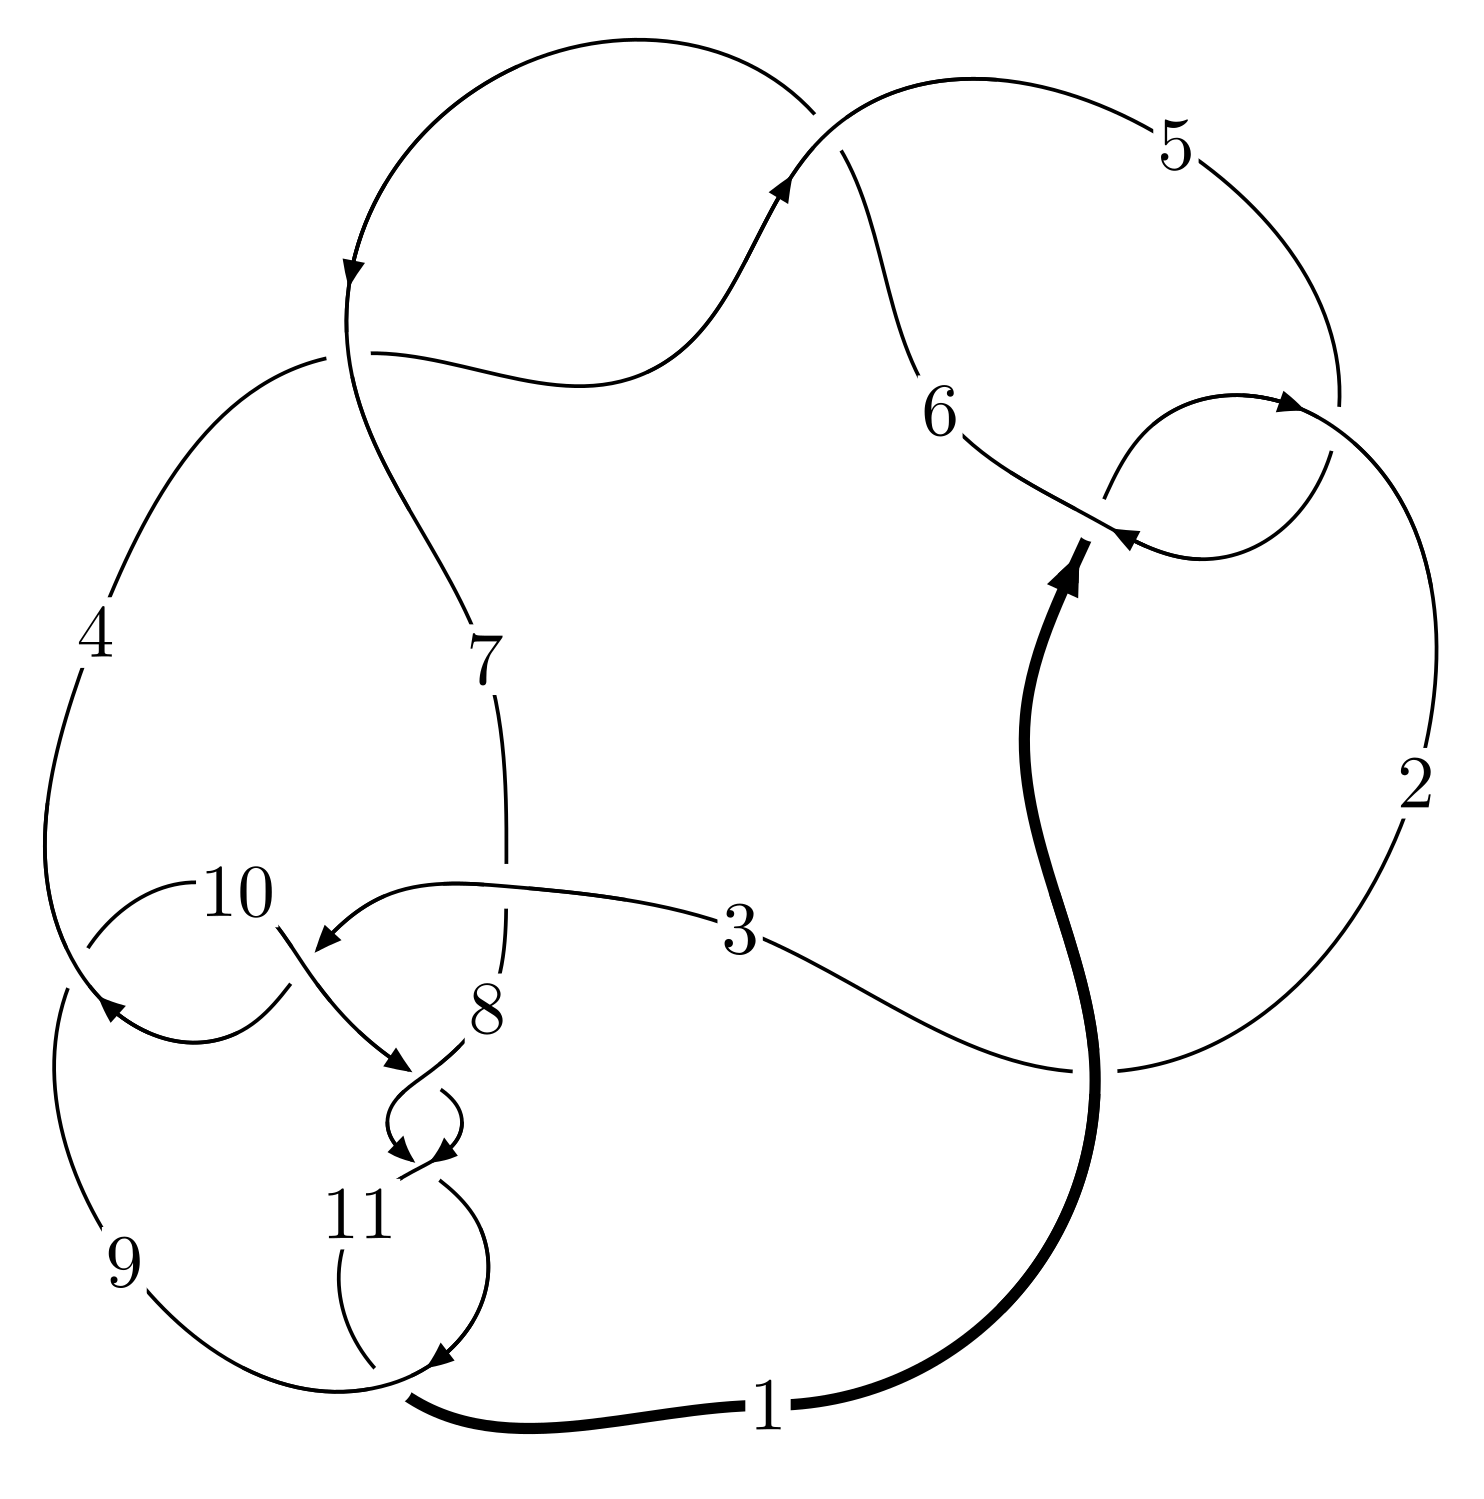
\includegraphics[width=112pt]{../../../GIT/diagram.site/Diagrams/png/367_11a_118.png}\\
\ \ \ A knot diagram\footnotemark}&
\allowdisplaybreaks
\textbf{Linearized knot diagam} \\
\cline{2-2}
 &
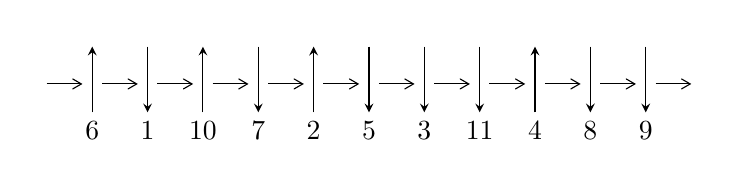
\begin{tikzpicture}[x=20pt, y=17pt]
	% nodes
	\node (C0) at (0, 0) {};
	\node (C1) at (1, 0) {};
	\node (C1U) at (1, +1) {};
	\node (C1D) at (1, -1) {6};

	\node (C2) at (2, 0) {};
	\node (C2U) at (2, +1) {};
	\node (C2D) at (2, -1) {1};

	\node (C3) at (3, 0) {};
	\node (C3U) at (3, +1) {};
	\node (C3D) at (3, -1) {10};

	\node (C4) at (4, 0) {};
	\node (C4U) at (4, +1) {};
	\node (C4D) at (4, -1) {7};

	\node (C5) at (5, 0) {};
	\node (C5U) at (5, +1) {};
	\node (C5D) at (5, -1) {2};

	\node (C6) at (6, 0) {};
	\node (C6U) at (6, +1) {};
	\node (C6D) at (6, -1) {5};

	\node (C7) at (7, 0) {};
	\node (C7U) at (7, +1) {};
	\node (C7D) at (7, -1) {3};

	\node (C8) at (8, 0) {};
	\node (C8U) at (8, +1) {};
	\node (C8D) at (8, -1) {11};

	\node (C9) at (9, 0) {};
	\node (C9U) at (9, +1) {};
	\node (C9D) at (9, -1) {4};

	\node (C10) at (10, 0) {};
	\node (C10U) at (10, +1) {};
	\node (C10D) at (10, -1) {8};

	\node (C11) at (11, 0) {};
	\node (C11U) at (11, +1) {};
	\node (C11D) at (11, -1) {9};
	\node (C12) at (12, 0) {};

	% arrows
	\draw[->,>={angle 60}]
	(C0) edge (C1) (C1) edge (C2) (C2) edge (C3) (C3) edge (C4) (C4) edge (C5) (C5) edge (C6) (C6) edge (C7) (C7) edge (C8) (C8) edge (C9) (C9) edge (C10) (C10) edge (C11) (C11) edge (C12) ;	\draw[->,>=stealth]
	(C1D) edge (C1U) (C2U) edge (C2D) (C3D) edge (C3U) (C4U) edge (C4D) (C5D) edge (C5U) (C6U) edge (C6D) (C7U) edge (C7D) (C8U) edge (C8D) (C9D) edge (C9U) (C10U) edge (C10D) (C11U) edge (C11D) ;
	\end{tikzpicture} \\
\hhline{~~} \\& 
\textbf{Solving Sequence} \\ \cline{2-2} 
 &
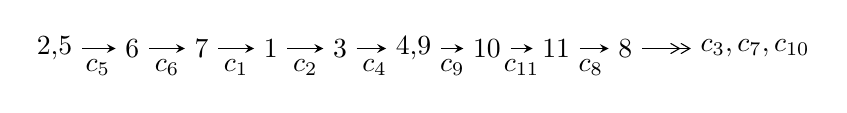
\begin{tikzpicture}[x=25pt, y=7pt]
	% node
	\node (A0) at (-1/8, 0) {2,5};
	\node (A1) at (1, 0) {6};
	\node (A2) at (2, 0) {7};
	\node (A3) at (3, 0) {1};
	\node (A4) at (4, 0) {3};
	\node (A5) at (81/16, 0) {4,9};
	\node (A6) at (49/8, 0) {10};
	\node (A7) at (57/8, 0) {11};
	\node (A8) at (65/8, 0) {8};
	\node (C1) at (1/2, -1) {$c_{5}$};
	\node (C2) at (3/2, -1) {$c_{6}$};
	\node (C3) at (5/2, -1) {$c_{1}$};
	\node (C4) at (7/2, -1) {$c_{2}$};
	\node (C5) at (9/2, -1) {$c_{4}$};
	\node (C6) at (45/8, -1) {$c_{9}$};
	\node (C7) at (53/8, -1) {$c_{11}$};
	\node (C8) at (61/8, -1) {$c_{8}$};
	\node (A9) at (10, 0) {$c_{3},c_{7},c_{10}$};

	% edge
	\draw[->,>=stealth]	
	(A0) edge (A1) (A1) edge (A2) (A2) edge (A3) (A3) edge (A4) (A4) edge (A5) (A5) edge (A6) (A6) edge (A7) (A7) edge (A8) ;
	\draw[->>,>={angle 60}]	
	(A8) edge (A9);
\end{tikzpicture} \\ 

\end{tabular} \\

\footnotetext{
The image of knot diagram is generated by the software ``\textbf{Draw programme}" developed by Andrew Bartholomew(\url{http://www.layer8.co.uk/maths/draw/index.htm\#Running-draw}), where we modified some parts for our purpose(\url{https://github.com/CATsTAILs/LinksPainter}).
}\phantom \\ \newline 
\centering \textbf{Ideals for irreducible components\footnotemark of $X_{\text{par}}$} 
 
\begin{align*}
I^u_{1}&=\langle 
2 u^{46}-4 u^{45}+\cdots+b+2,\;-2 u^{46}+2 u^{45}+\cdots+a+u,\;u^{47}-2 u^{46}+\cdots-2 u^2-1\rangle \\
I^u_{2}&=\langle 
u^2+b,\;a+u,\;u^4+u^3+u^2+1\rangle \\
\\
\end{align*}
\raggedright * 2 irreducible components of $\dim_{\mathbb{C}}=0$, with total 51 representations.\\
\footnotetext{All coefficients of polynomials are rational numbers. But the coefficients are sometimes approximated in decimal forms when there is not enough margin.}
\newpage
\renewcommand{\arraystretch}{1}
\centering \section*{I. $I^u_{1}= \langle 2 u^{46}-4 u^{45}+\cdots+b+2,\;-2 u^{46}+2 u^{45}+\cdots+a+u,\;u^{47}-2 u^{46}+\cdots-2 u^2-1 \rangle$}
\flushleft \textbf{(i) Arc colorings}\\
\begin{tabular}{m{7pt} m{180pt} m{7pt} m{180pt} }
\flushright $a_{2}=$&$\begin{pmatrix}0\\u\end{pmatrix}$ \\
\flushright $a_{5}=$&$\begin{pmatrix}1\\0\end{pmatrix}$ \\
\flushright $a_{6}=$&$\begin{pmatrix}1\\- u^2\end{pmatrix}$ \\
\flushright $a_{7}=$&$\begin{pmatrix}u^2+1\\- u^2\end{pmatrix}$ \\
\flushright $a_{1}=$&$\begin{pmatrix}- u\\u^3+u\end{pmatrix}$ \\
\flushright $a_{3}=$&$\begin{pmatrix}- u^3\\u^5+u^3+u\end{pmatrix}$ \\
\flushright $a_{4}=$&$\begin{pmatrix}u^4+u^2+1\\- u^4\end{pmatrix}$ \\
\flushright $a_{9}=$&$\begin{pmatrix}2 u^{46}-2 u^{45}+\cdots-10 u^3- u\\-2 u^{46}+4 u^{45}+\cdots-4 u^2-2\end{pmatrix}$ \\
\flushright $a_{10}=$&$\begin{pmatrix}- u^{42}-5 u^{40}+\cdots- u^2-1\\u^{43}+5 u^{41}+\cdots+u^3+u\end{pmatrix}$ \\
\flushright $a_{11}=$&$\begin{pmatrix}- u^{46}+u^{45}+\cdots+u^2+1\\u^{46}-2 u^{45}+\cdots+2 u^2+1\end{pmatrix}$ \\
\flushright $a_{8}=$&$\begin{pmatrix}- u^{10}- u^8-2 u^6- u^4+u^2+1\\u^{12}+2 u^{10}+4 u^8+4 u^6+3 u^4\end{pmatrix}$\\ \flushright $a_{8}=$&$\begin{pmatrix}- u^{10}- u^8-2 u^6- u^4+u^2+1\\u^{12}+2 u^{10}+4 u^8+4 u^6+3 u^4\end{pmatrix}$\\&\end{tabular}
\flushleft \textbf{(ii) Obstruction class $= -1$}\\~\\
\flushleft \textbf{(iii) Cusp Shapes $= 4 u^{46}-4 u^{45}+\cdots-13 u-5$}\\~\\
\newpage\renewcommand{\arraystretch}{1}
\flushleft \textbf{(iv) u-Polynomials at the component}\newline \\
\begin{tabular}{m{50pt}|m{274pt}}
Crossings & \hspace{64pt}u-Polynomials at each crossing \\
\hline $$\begin{aligned}c_{1},c_{5}\end{aligned}$$&$\begin{aligned}
&u^{47}-2 u^{46}+\cdots-2 u^2-1
\end{aligned}$\\
\hline $$\begin{aligned}c_{2},c_{4},c_{6}\end{aligned}$$&$\begin{aligned}
&u^{47}+12 u^{46}+\cdots-4 u-1
\end{aligned}$\\
\hline $$\begin{aligned}c_{3},c_{9}\end{aligned}$$&$\begin{aligned}
&u^{47}- u^{46}+\cdots+56 u+16
\end{aligned}$\\
\hline $$\begin{aligned}c_{7}\end{aligned}$$&$\begin{aligned}
&u^{47}-2 u^{46}+\cdots+692 u-241
\end{aligned}$\\
\hline $$\begin{aligned}c_{8},c_{10},c_{11}\end{aligned}$$&$\begin{aligned}
&u^{47}-5 u^{46}+\cdots-2 u+1
\end{aligned}$\\
\hline
\end{tabular}\\~\\
\newpage\renewcommand{\arraystretch}{1}
\flushleft \textbf{(v) Riley Polynomials at the component}\newline \\
\begin{tabular}{m{50pt}|m{274pt}}
Crossings & \hspace{64pt}Riley Polynomials at each crossing \\
\hline $$\begin{aligned}c_{1},c_{5}\end{aligned}$$&$\begin{aligned}
&y^{47}+12 y^{46}+\cdots-4 y-1
\end{aligned}$\\
\hline $$\begin{aligned}c_{2},c_{4},c_{6}\end{aligned}$$&$\begin{aligned}
&y^{47}+48 y^{46}+\cdots+20 y-1
\end{aligned}$\\
\hline $$\begin{aligned}c_{3},c_{9}\end{aligned}$$&$\begin{aligned}
&y^{47}+27 y^{46}+\cdots-1472 y-256
\end{aligned}$\\
\hline $$\begin{aligned}c_{7}\end{aligned}$$&$\begin{aligned}
&y^{47}-12 y^{46}+\cdots-623952 y-58081
\end{aligned}$\\
\hline $$\begin{aligned}c_{8},c_{10},c_{11}\end{aligned}$$&$\begin{aligned}
&y^{47}-45 y^{46}+\cdots-14 y-1
\end{aligned}$\\
\hline
\end{tabular}\\~\\
\newpage\flushleft \textbf{(vi) Complex Volumes and Cusp Shapes}
$$\begin{array}{c|c|c}  
\text{Solutions to }I^u_{1}& \I (\text{vol} + \sqrt{-1}CS) & \text{Cusp shape}\\
 \hline 
\begin{aligned}
u &= -0.323780 + 0.951481 I \\
a &= -1.040000 - 0.645980 I \\
b &= \phantom{-}0.039385 + 0.152748 I\end{aligned}
 & -2.98908 - 5.01589 I & -7.64324 + 7.88279 I \\ \hline\begin{aligned}
u &= -0.323780 - 0.951481 I \\
a &= -1.040000 + 0.645980 I \\
b &= \phantom{-}0.039385 - 0.152748 I\end{aligned}
 & -2.98908 + 5.01589 I & -7.64324 - 7.88279 I \\ \hline\begin{aligned}
u &= \phantom{-}0.279046 + 0.946930 I \\
a &= \phantom{-}0.56107 - 1.31422 I \\
b &= -1.13319 + 1.30432 I\end{aligned}
 & -5.33668 + 2.70197 I & -9.52160 - 4.32403 I \\ \hline\begin{aligned}
u &= \phantom{-}0.279046 - 0.946930 I \\
a &= \phantom{-}0.56107 + 1.31422 I \\
b &= -1.13319 - 1.30432 I\end{aligned}
 & -5.33668 - 2.70197 I & -9.52160 + 4.32403 I \\ \hline\begin{aligned}
u &= -0.162628 + 1.011340 I \\
a &= -0.246189 + 0.321696 I \\
b &= -0.52431 - 1.50699 I\end{aligned}
 & -10.43430 + 2.59019 I & -12.08721 - 0.43654 I \\ \hline\begin{aligned}
u &= -0.162628 - 1.011340 I \\
a &= -0.246189 - 0.321696 I \\
b &= -0.52431 + 1.50699 I\end{aligned}
 & -10.43430 - 2.59019 I & -12.08721 + 0.43654 I \\ \hline\begin{aligned}
u &= -0.228159 + 0.924111 I \\
a &= \phantom{-}0.482803 + 0.476440 I \\
b &= \phantom{-}0.496433 + 0.569748 I\end{aligned}
 & -3.55919 - 0.29784 I & -10.26703 + 0.71916 I \\ \hline\begin{aligned}
u &= -0.228159 - 0.924111 I \\
a &= \phantom{-}0.482803 - 0.476440 I \\
b &= \phantom{-}0.496433 - 0.569748 I\end{aligned}
 & -3.55919 + 0.29784 I & -10.26703 - 0.71916 I \\ \hline\begin{aligned}
u &= \phantom{-}0.708344 + 0.612950 I \\
a &= -0.171277 - 1.044900 I \\
b &= \phantom{-}0.358664 + 0.237870 I\end{aligned}
 & -4.59202 + 2.73053 I & -5.50356 - 3.27752 I \\ \hline\begin{aligned}
u &= \phantom{-}0.708344 - 0.612950 I \\
a &= -0.171277 + 1.044900 I \\
b &= \phantom{-}0.358664 - 0.237870 I\end{aligned}
 & -4.59202 - 2.73053 I & -5.50356 + 3.27752 I\\
 \hline 
 \end{array}$$\newpage$$\begin{array}{c|c|c}  
\text{Solutions to }I^u_{1}& \I (\text{vol} + \sqrt{-1}CS) & \text{Cusp shape}\\
 \hline 
\begin{aligned}
u &= -0.356410 + 1.011910 I \\
a &= \phantom{-}1.41420 + 0.68105 I \\
b &= -0.864275 - 0.447765 I\end{aligned}
 & -9.29934 - 8.73167 I & -9.77244 + 7.33268 I \\ \hline\begin{aligned}
u &= -0.356410 - 1.011910 I \\
a &= \phantom{-}1.41420 - 0.68105 I \\
b &= -0.864275 + 0.447765 I\end{aligned}
 & -9.29934 + 8.73167 I & -9.77244 - 7.33268 I \\ \hline\begin{aligned}
u &= \phantom{-}0.340688 + 0.794423 I \\
a &= -0.122254 + 0.637267 I \\
b &= \phantom{-}0.278704 - 0.519560 I\end{aligned}
 & -0.34710 + 1.73528 I & -0.42828 - 4.75697 I \\ \hline\begin{aligned}
u &= \phantom{-}0.340688 - 0.794423 I \\
a &= -0.122254 - 0.637267 I \\
b &= \phantom{-}0.278704 + 0.519560 I\end{aligned}
 & -0.34710 - 1.73528 I & -0.42828 + 4.75697 I \\ \hline\begin{aligned}
u &= \phantom{-}0.683839 + 0.940887 I \\
a &= -0.548528 - 0.398362 I \\
b &= \phantom{-}0.617662 - 0.068827 I\end{aligned}
 & -5.43573 + 2.43943 I & -7.50586 - 2.89264 I \\ \hline\begin{aligned}
u &= \phantom{-}0.683839 - 0.940887 I \\
a &= -0.548528 + 0.398362 I \\
b &= \phantom{-}0.617662 + 0.068827 I\end{aligned}
 & -5.43573 - 2.43943 I & -7.50586 + 2.89264 I \\ \hline\begin{aligned}
u &= -0.834781 + 0.823539 I \\
a &= \phantom{-}1.25208 + 1.37561 I \\
b &= -2.22075 + 1.02814 I\end{aligned}
 & \phantom{-}1.68842 + 0.66706 I & -2.90341 + 0. I\phantom{ +0.000000I} \\ \hline\begin{aligned}
u &= -0.834781 - 0.823539 I \\
a &= \phantom{-}1.25208 - 1.37561 I \\
b &= -2.22075 - 1.02814 I\end{aligned}
 & \phantom{-}1.68842 - 0.66706 I & -2.90341 + 0. I\phantom{ +0.000000I} \\ \hline\begin{aligned}
u &= \phantom{-}0.815351 + 0.845486 I \\
a &= \phantom{-}1.63790 + 0.06363 I \\
b &= -1.65919 - 1.45595 I\end{aligned}
 & \phantom{-}2.81443 + 1.97841 I & -3.90653 - 2.24549 I \\ \hline\begin{aligned}
u &= \phantom{-}0.815351 - 0.845486 I \\
a &= \phantom{-}1.63790 - 0.06363 I \\
b &= -1.65919 + 1.45595 I\end{aligned}
 & \phantom{-}2.81443 - 1.97841 I & -3.90653 + 2.24549 I\\
 \hline 
 \end{array}$$\newpage$$\begin{array}{c|c|c}  
\text{Solutions to }I^u_{1}& \I (\text{vol} + \sqrt{-1}CS) & \text{Cusp shape}\\
 \hline 
\begin{aligned}
u &= \phantom{-}0.857523 + 0.824218 I \\
a &= -1.55042 + 1.32128 I \\
b &= \phantom{-}2.82438 + 0.47847 I\end{aligned}
 & \phantom{-}4.54046 - 2.88310 I & -0.74757 + 2.68199 I \\ \hline\begin{aligned}
u &= \phantom{-}0.857523 - 0.824218 I \\
a &= -1.55042 - 1.32128 I \\
b &= \phantom{-}2.82438 - 0.47847 I\end{aligned}
 & \phantom{-}4.54046 + 2.88310 I & -0.74757 - 2.68199 I \\ \hline\begin{aligned}
u &= \phantom{-}0.885800 + 0.806423 I \\
a &= \phantom{-}0.87468 - 2.17600 I \\
b &= -3.02165 + 0.59943 I\end{aligned}
 & -1.16589 - 7.05931 I & -3.99587 + 3.23207 I \\ \hline\begin{aligned}
u &= \phantom{-}0.885800 - 0.806423 I \\
a &= \phantom{-}0.87468 + 2.17600 I \\
b &= -3.02165 - 0.59943 I\end{aligned}
 & -1.16589 + 7.05931 I & -3.99587 - 3.23207 I \\ \hline\begin{aligned}
u &= -0.846893 + 0.876661 I \\
a &= -1.243050 - 0.582712 I \\
b &= \phantom{-}1.61840 - 1.14508 I\end{aligned}
 & \phantom{-}6.78103 - 1.89076 I & \phantom{-}3.32003 + 1.86990 I \\ \hline\begin{aligned}
u &= -0.846893 - 0.876661 I \\
a &= -1.243050 + 0.582712 I \\
b &= \phantom{-}1.61840 + 1.14508 I\end{aligned}
 & \phantom{-}6.78103 + 1.89076 I & \phantom{-}3.32003 - 1.86990 I \\ \hline\begin{aligned}
u &= \phantom{-}0.789107 + 0.937549 I \\
a &= -0.18516 + 1.60290 I \\
b &= \phantom{-}1.69367 - 0.69541 I\end{aligned}
 & \phantom{-}2.52856 + 4.03641 I & -4.47860 - 2.87730 I \\ \hline\begin{aligned}
u &= \phantom{-}0.789107 - 0.937549 I \\
a &= -0.18516 - 1.60290 I \\
b &= \phantom{-}1.69367 + 0.69541 I\end{aligned}
 & \phantom{-}2.52856 - 4.03641 I & -4.47860 + 2.87730 I \\ \hline\begin{aligned}
u &= -0.793086 + 0.958197 I \\
a &= -1.31875 - 1.11688 I \\
b &= \phantom{-}3.24344 - 0.25353 I\end{aligned}
 & \phantom{-}1.27181 - 6.75017 I & -3.82680 + 4.90142 I \\ \hline\begin{aligned}
u &= -0.793086 - 0.958197 I \\
a &= -1.31875 + 1.11688 I \\
b &= \phantom{-}3.24344 + 0.25353 I\end{aligned}
 & \phantom{-}1.27181 + 6.75017 I & -3.82680 - 4.90142 I\\
 \hline 
 \end{array}$$\newpage$$\begin{array}{c|c|c}  
\text{Solutions to }I^u_{1}& \I (\text{vol} + \sqrt{-1}CS) & \text{Cusp shape}\\
 \hline 
\begin{aligned}
u &= -0.827450 + 0.929808 I \\
a &= \phantom{-}0.652950 + 1.101310 I \\
b &= -2.09248 - 0.31110 I\end{aligned}
 & \phantom{-}6.61449 - 4.34054 I & \phantom{-}3.06304 + 3.52446 I \\ \hline\begin{aligned}
u &= -0.827450 - 0.929808 I \\
a &= \phantom{-}0.652950 - 1.101310 I \\
b &= -2.09248 + 0.31110 I\end{aligned}
 & \phantom{-}6.61449 + 4.34054 I & \phantom{-}3.06304 - 3.52446 I \\ \hline\begin{aligned}
u &= \phantom{-}0.805855 + 0.968008 I \\
a &= \phantom{-}1.48174 - 1.44769 I \\
b &= -2.97050 - 0.63587 I\end{aligned}
 & \phantom{-}4.09177 + 9.07422 I & \phantom{-0.000000 } 0. - 7.57119 I \\ \hline\begin{aligned}
u &= \phantom{-}0.805855 - 0.968008 I \\
a &= \phantom{-}1.48174 + 1.44769 I \\
b &= -2.97050 + 0.63587 I\end{aligned}
 & \phantom{-}4.09177 - 9.07422 I & \phantom{-0.000000 -}0. + 7.57119 I \\ \hline\begin{aligned}
u &= -0.880114 + 0.921081 I \\
a &= \phantom{-}1.22606 - 1.28739 I \\
b &= \phantom{-}0.27179 + 2.45585 I\end{aligned}
 & \phantom{-}4.07979 - 3.25139 I & -6.94110 + 0. I\phantom{ +0.000000I} \\ \hline\begin{aligned}
u &= -0.880114 - 0.921081 I \\
a &= \phantom{-}1.22606 + 1.28739 I \\
b &= \phantom{-}0.27179 - 2.45585 I\end{aligned}
 & \phantom{-}4.07979 + 3.25139 I & -6.94110 + 0. I\phantom{ +0.000000I} \\ \hline\begin{aligned}
u &= \phantom{-}0.811281 + 0.991380 I \\
a &= -2.18383 + 0.73777 I \\
b &= \phantom{-}3.18948 + 1.96415 I\end{aligned}
 & -1.74737 + 13.34970 I & \phantom{-0.000000 } 0. - 7.91325 I \\ \hline\begin{aligned}
u &= \phantom{-}0.811281 - 0.991380 I \\
a &= -2.18383 - 0.73777 I \\
b &= \phantom{-}3.18948 - 1.96415 I\end{aligned}
 & -1.74737 - 13.34970 I & \phantom{-0.000000 -}0. + 7.91325 I \\ \hline\begin{aligned}
u &= -0.689977 + 0.164527 I \\
a &= -1.53731 - 0.89142 I \\
b &= \phantom{-}0.350409 + 0.785923 I\end{aligned}
 & -6.58964 + 5.02938 I & -4.60471 - 3.19808 I \\ \hline\begin{aligned}
u &= -0.689977 - 0.164527 I \\
a &= -1.53731 + 0.89142 I \\
b &= \phantom{-}0.350409 - 0.785923 I\end{aligned}
 & -6.58964 - 5.02938 I & -4.60471 + 3.19808 I\\
 \hline 
 \end{array}$$\newpage$$\begin{array}{c|c|c}  
\text{Solutions to }I^u_{1}& \I (\text{vol} + \sqrt{-1}CS) & \text{Cusp shape}\\
 \hline 
\begin{aligned}
u &= \phantom{-}0.412032 + 0.515876 I \\
a &= \phantom{-}1.082960 + 0.365898 I \\
b &= -0.467743 - 0.314327 I\end{aligned}
 & \phantom{-}0.483129 + 1.240200 I & \phantom{-}2.11511 - 5.50878 I \\ \hline\begin{aligned}
u &= \phantom{-}0.412032 - 0.515876 I \\
a &= \phantom{-}1.082960 - 0.365898 I \\
b &= -0.467743 + 0.314327 I\end{aligned}
 & \phantom{-}0.483129 - 1.240200 I & \phantom{-}2.11511 + 5.50878 I \\ \hline\begin{aligned}
u &= -0.160236 + 0.579743 I \\
a &= -1.03520 + 1.13349 I \\
b &= \phantom{-}0.691220 + 0.719972 I\end{aligned}
 & -2.00613 - 0.73127 I & -7.95587 - 2.97532 I \\ \hline\begin{aligned}
u &= -0.160236 - 0.579743 I \\
a &= -1.03520 - 1.13349 I \\
b &= \phantom{-}0.691220 - 0.719972 I\end{aligned}
 & -2.00613 + 0.73127 I & -7.95587 + 2.97532 I \\ \hline\begin{aligned}
u &= -0.532528 + 0.151857 I \\
a &= \phantom{-}0.891221 - 0.043389 I \\
b &= -0.132594 - 0.683828 I\end{aligned}
 & -0.60484 + 1.87329 I & -1.11748 - 3.89488 I \\ \hline\begin{aligned}
u &= -0.532528 - 0.151857 I \\
a &= \phantom{-}0.891221 + 0.043389 I \\
b &= -0.132594 + 0.683828 I\end{aligned}
 & -0.60484 - 1.87329 I & -1.11748 + 3.89488 I \\ \hline\begin{aligned}
u &= \phantom{-}0.494353\phantom{ +0.000000I} \\
a &= -2.75136\phantom{ +0.000000I} \\
b &= \phantom{-}0.826082\phantom{ +0.000000I}\end{aligned}
 & -2.69658\phantom{ +0.000000I} & -2.16950\phantom{ +0.000000I}\\
 \hline 
 \end{array}$$\newpage\newpage\renewcommand{\arraystretch}{1}
\centering \section*{II. $I^u_{2}= \langle u^2+b,\;a+u,\;u^4+u^3+u^2+1 \rangle$}
\flushleft \textbf{(i) Arc colorings}\\
\begin{tabular}{m{7pt} m{180pt} m{7pt} m{180pt} }
\flushright $a_{2}=$&$\begin{pmatrix}0\\u\end{pmatrix}$ \\
\flushright $a_{5}=$&$\begin{pmatrix}1\\0\end{pmatrix}$ \\
\flushright $a_{6}=$&$\begin{pmatrix}1\\- u^2\end{pmatrix}$ \\
\flushright $a_{7}=$&$\begin{pmatrix}u^2+1\\- u^2\end{pmatrix}$ \\
\flushright $a_{1}=$&$\begin{pmatrix}- u\\u^3+u\end{pmatrix}$ \\
\flushright $a_{3}=$&$\begin{pmatrix}- u^3\\u^3+u^2+1\end{pmatrix}$ \\
\flushright $a_{4}=$&$\begin{pmatrix}- u^3\\u^3+u^2+1\end{pmatrix}$ \\
\flushright $a_{9}=$&$\begin{pmatrix}- u\\- u^2\end{pmatrix}$ \\
\flushright $a_{10}=$&$\begin{pmatrix}- u\\- u^2\end{pmatrix}$ \\
\flushright $a_{11}=$&$\begin{pmatrix}-2 u\\u^3- u^2+u\end{pmatrix}$ \\
\flushright $a_{8}=$&$\begin{pmatrix}u\\- u^3- u\end{pmatrix}$\\ \flushright $a_{8}=$&$\begin{pmatrix}u\\- u^3- u\end{pmatrix}$\\&\end{tabular}
\flushleft \textbf{(ii) Obstruction class $= 1$}\\~\\
\flushleft \textbf{(iii) Cusp Shapes $= -5 u^2-6 u-5$}\\~\\
\newpage\renewcommand{\arraystretch}{1}
\flushleft \textbf{(iv) u-Polynomials at the component}\newline \\
\begin{tabular}{m{50pt}|m{274pt}}
Crossings & \hspace{64pt}u-Polynomials at each crossing \\
\hline $$\begin{aligned}c_{1}\end{aligned}$$&$\begin{aligned}
&u^4- u^3+u^2+1
\end{aligned}$\\
\hline $$\begin{aligned}c_{2},c_{6},c_{7}\end{aligned}$$&$\begin{aligned}
&u^4+u^3+3 u^2+2 u+1
\end{aligned}$\\
\hline $$\begin{aligned}c_{3},c_{9}\end{aligned}$$&$\begin{aligned}
&u^4
\end{aligned}$\\
\hline $$\begin{aligned}c_{4}\end{aligned}$$&$\begin{aligned}
&u^4- u^3+3 u^2-2 u+1
\end{aligned}$\\
\hline $$\begin{aligned}c_{5}\end{aligned}$$&$\begin{aligned}
&u^4+u^3+u^2+1
\end{aligned}$\\
\hline $$\begin{aligned}c_{8}\end{aligned}$$&$\begin{aligned}
&(u-1)^4
\end{aligned}$\\
\hline $$\begin{aligned}c_{10},c_{11}\end{aligned}$$&$\begin{aligned}
&(u+1)^4
\end{aligned}$\\
\hline
\end{tabular}\\~\\
\newpage\renewcommand{\arraystretch}{1}
\flushleft \textbf{(v) Riley Polynomials at the component}\newline \\
\begin{tabular}{m{50pt}|m{274pt}}
Crossings & \hspace{64pt}Riley Polynomials at each crossing \\
\hline $$\begin{aligned}c_{1},c_{5}\end{aligned}$$&$\begin{aligned}
&y^4+y^3+3 y^2+2 y+1
\end{aligned}$\\
\hline $$\begin{aligned}c_{2},c_{4},c_{6}\\c_{7}\end{aligned}$$&$\begin{aligned}
&y^4+5 y^3+7 y^2+2 y+1
\end{aligned}$\\
\hline $$\begin{aligned}c_{3},c_{9}\end{aligned}$$&$\begin{aligned}
&y^4
\end{aligned}$\\
\hline $$\begin{aligned}c_{8},c_{10},c_{11}\end{aligned}$$&$\begin{aligned}
&(y-1)^4
\end{aligned}$\\
\hline
\end{tabular}\\~\\
\newpage\flushleft \textbf{(vi) Complex Volumes and Cusp Shapes}
$$\begin{array}{c|c|c}  
\text{Solutions to }I^u_{2}& \I (\text{vol} + \sqrt{-1}CS) & \text{Cusp shape}\\
 \hline 
\begin{aligned}
u &= \phantom{-}0.351808 + 0.720342 I \\
a &= -0.351808 - 0.720342 I \\
b &= \phantom{-}0.395123 - 0.506844 I\end{aligned}
 & -1.85594 + 1.41510 I & -5.13523 - 6.85627 I \\ \hline\begin{aligned}
u &= \phantom{-}0.351808 - 0.720342 I \\
a &= -0.351808 + 0.720342 I \\
b &= \phantom{-}0.395123 + 0.506844 I\end{aligned}
 & -1.85594 - 1.41510 I & -5.13523 + 6.85627 I \\ \hline\begin{aligned}
u &= -0.851808 + 0.911292 I \\
a &= \phantom{-}0.851808 - 0.911292 I \\
b &= \phantom{-}0.10488 + 1.55249 I\end{aligned}
 & \phantom{-}5.14581 - 3.16396 I & \phantom{-}0.63523 + 2.29471 I \\ \hline\begin{aligned}
u &= -0.851808 - 0.911292 I \\
a &= \phantom{-}0.851808 + 0.911292 I \\
b &= \phantom{-}0.10488 - 1.55249 I\end{aligned}
 & \phantom{-}5.14581 + 3.16396 I & \phantom{-}0.63523 - 2.29471 I\\
 \hline 
 \end{array}$$\newpage
\newpage\renewcommand{\arraystretch}{1}
\centering \section*{ III. u-Polynomials}
\begin{tabular}{m{50pt}|m{274pt}}
Crossings & \hspace{64pt}u-Polynomials at each crossing \\
\hline $$\begin{aligned}c_{1}\end{aligned}$$&$\begin{aligned}
&(u^4- u^3+u^2+1)(u^{47}-2 u^{46}+\cdots-2 u^2-1)
\end{aligned}$\\
\hline $$\begin{aligned}c_{2},c_{6}\end{aligned}$$&$\begin{aligned}
&(u^4+u^3+3 u^2+2 u+1)(u^{47}+12 u^{46}+\cdots-4 u-1)
\end{aligned}$\\
\hline $$\begin{aligned}c_{3},c_{9}\end{aligned}$$&$\begin{aligned}
&u^4(u^{47}- u^{46}+\cdots+56 u+16)
\end{aligned}$\\
\hline $$\begin{aligned}c_{4}\end{aligned}$$&$\begin{aligned}
&(u^4- u^3+3 u^2-2 u+1)(u^{47}+12 u^{46}+\cdots-4 u-1)
\end{aligned}$\\
\hline $$\begin{aligned}c_{5}\end{aligned}$$&$\begin{aligned}
&(u^4+u^3+u^2+1)(u^{47}-2 u^{46}+\cdots-2 u^2-1)
\end{aligned}$\\
\hline $$\begin{aligned}c_{7}\end{aligned}$$&$\begin{aligned}
&(u^4+u^3+3 u^2+2 u+1)(u^{47}-2 u^{46}+\cdots+692 u-241)
\end{aligned}$\\
\hline $$\begin{aligned}c_{8}\end{aligned}$$&$\begin{aligned}
&((u-1)^4)(u^{47}-5 u^{46}+\cdots-2 u+1)
\end{aligned}$\\
\hline $$\begin{aligned}c_{10},c_{11}\end{aligned}$$&$\begin{aligned}
&((u+1)^4)(u^{47}-5 u^{46}+\cdots-2 u+1)
\end{aligned}$\\
\hline
\end{tabular}\newpage\renewcommand{\arraystretch}{1}
\centering \section*{ IV. Riley Polynomials}
\begin{tabular}{m{50pt}|m{274pt}}
Crossings & \hspace{64pt}Riley Polynomials at each crossing \\
\hline $$\begin{aligned}c_{1},c_{5}\end{aligned}$$&$\begin{aligned}
&(y^4+y^3+3 y^2+2 y+1)(y^{47}+12 y^{46}+\cdots-4 y-1)
\end{aligned}$\\
\hline $$\begin{aligned}c_{2},c_{4},c_{6}\end{aligned}$$&$\begin{aligned}
&(y^4+5 y^3+7 y^2+2 y+1)(y^{47}+48 y^{46}+\cdots+20 y-1)
\end{aligned}$\\
\hline $$\begin{aligned}c_{3},c_{9}\end{aligned}$$&$\begin{aligned}
&y^4(y^{47}+27 y^{46}+\cdots-1472 y-256)
\end{aligned}$\\
\hline $$\begin{aligned}c_{7}\end{aligned}$$&$\begin{aligned}
&(y^4+5 y^3+7 y^2+2 y+1)(y^{47}-12 y^{46}+\cdots-623952 y-58081)
\end{aligned}$\\
\hline $$\begin{aligned}c_{8},c_{10},c_{11}\end{aligned}$$&$\begin{aligned}
&((y-1)^4)(y^{47}-45 y^{46}+\cdots-14 y-1)
\end{aligned}$\\
\hline
\end{tabular}
\vskip 2pc
\end{document}